\chapter{Introduction to Computational Science}

\section{Learning Objectives}

Upon completion of this chapter, students should be able to:

\begin{enumerate}
  \item Define computational science and explain its interdisciplinary nature
  \item Identify the three pillars of computational science and understand their interconnected relationship
  \item Understand the role of computational thinking in problem-solving across various domains
  \item Recognize applications of computational science across diverse fields including physics, biology, economics, and engineering
  \item Distinguish between different types of computational models and their appropriate applications
  \item Explain the computational science workflow and methodology for systematic problem-solving
  \item Appreciate the tripartite approach that distinguishes computational science from traditional scientific methods
  \item Understand how computational science bridges theoretical and experimental approaches to scientific inquiry
\end{enumerate}

\begin{figure}[ht]
  \centering
  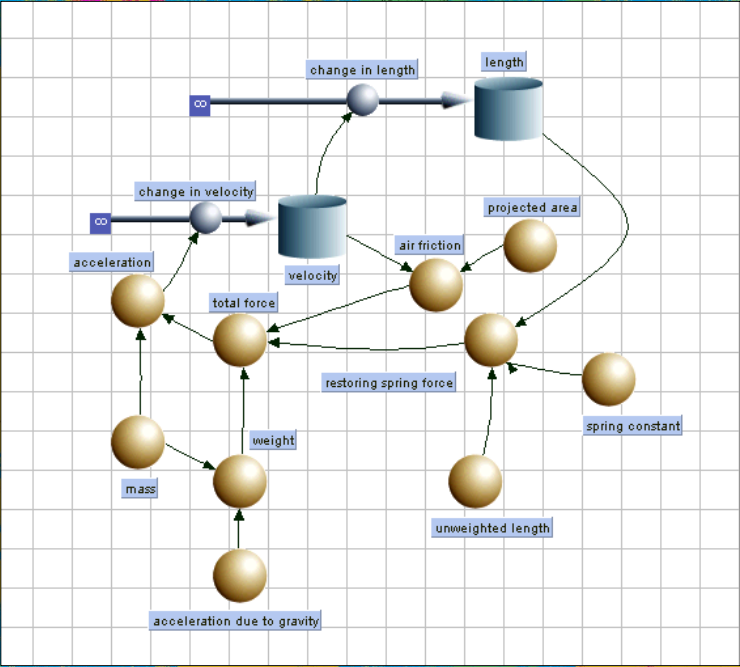
\includegraphics[width=0.8\textwidth]{images/chapter1_title_simulation.png}
  \caption{Mass-Spring Dynamics Simulation}
  \label{fig:chapter1_title}
\end{figure}

Figure~\ref{fig:chapter1_title} shows the computational modeling of a physical system with interconnected masses, springs, and forces including gravity, air friction, and restoring forces.

\section{Mass-Spring Dynamics Simulation}

\subsection{What is Mass-Spring Dynamics?}

\begin{conceptcard}{Mass-Spring Dynamics Definition}
\textbf{Mass-Spring Dynamics} is a fundamental physical and computational model that describes the behavior of systems consisting of point masses connected by elastic springs. This model serves as a cornerstone in physics, engineering, and computational science for understanding oscillatory motion, mechanical vibrations, and complex multi-body systems.
\end{conceptcard}

Mass-Spring Dynamics represents one of the most important and widely applicable models in computational physics. At its core, it describes how objects with mass respond to forces, particularly the restoring forces exerted by springs and the influence of external forces such as gravity and friction.

\subsubsection{Fundamental Components of Mass-Spring Systems}

A mass-spring system consists of several key elements that work together to create complex dynamic behaviors:

\begin{enumerate}
    \item \textbf{Point Masses}: These represent objects with mass but negligible size, characterized by:
    \begin{itemize}
        \item Mass value (m) that determines inertial properties
        \item Position coordinates (x, y, z) in space
        \item Velocity components that describe motion
        \item Acceleration determined by applied forces
    \end{itemize}
    
    \item \textbf{Springs}: Elastic connectors that exert forces proportional to displacement:
    \begin{itemize}
        \item Spring constant (k) indicating stiffness
        \item Natural (rest) length when no force is applied
        \item Current length based on connected mass positions
        \item Restoring force that opposes deformation
    \end{itemize}
    
    \item \textbf{External Forces}: Environmental influences affecting the system:
    \begin{itemize}
        \item Gravitational acceleration pulling masses downward
        \item Air resistance opposing motion
        \item Applied forces from user interaction or external sources
        \item Constraint forces maintaining system integrity
    \end{itemize}
    
    \item \textbf{Damping Elements}: Energy dissipation mechanisms:
    \begin{itemize}
        \item Viscous damping proportional to velocity
        \item Friction forces opposing motion
        \item Energy loss that causes oscillations to decay over time
    \end{itemize}
\end{enumerate}

\subsubsection{Physical Principles Governing Mass-Spring Dynamics}

The behavior of mass-spring systems is governed by fundamental laws of physics that can be expressed mathematically:

\begin{enumerate}
    \item \textbf{Newton's Second Law of Motion}:
    \begin{equation}
        \vec{F}_{net} = m\vec{a}
    \end{equation}
    where the net force on a mass determines its acceleration.
    
    \item \textbf{Hooke's Law for Elastic Springs}:
    \begin{equation}
        \vec{F}_{spring} = -k(\vec{L} - \vec{L_0})
    \end{equation}
    where:
    \begin{itemize}
        \item k is the spring constant (stiffness)
        \item $\vec{L}$ is the current spring vector
        \item $\vec{L_0}$ is the natural length vector
        \item The negative sign indicates the force opposes displacement
    \end{itemize}
    
    \item \textbf{Damping Forces}:
    \begin{equation}
        \vec{F}_{damping} = -c\vec{v}
    \end{equation}
    where c is the damping coefficient and $\vec{v}$ is the velocity vector.
    
    \item \textbf{Energy Conservation Principles}:
    \begin{itemize}
        \item Kinetic energy: $KE = \frac{1}{2}mv^2$
        \item Potential energy: $PE = \frac{1}{2}kx^2$ (for springs)
        \item Total mechanical energy in ideal systems without damping
    \end{itemize}
\end{enumerate}

\subsubsection{Applications of Mass-Spring Dynamics}

Mass-spring dynamics finds applications across numerous fields, making it a versatile and important computational model:

\begin{itemize}
    \item \textbf{Mechanical Engineering}:
    \begin{itemize}
        \item Vehicle suspension system design and analysis
        \item Vibration isolation in machinery and equipment
        \item Structural dynamics of buildings and bridges
        \item Shock absorber optimization
    \end{itemize}
    
    \item \textbf{Computer Graphics and Animation}:
    \begin{itemize}
        \item Realistic cloth and fabric simulation
        \item Hair and fur dynamics in character animation
        \item Soft body deformation in games and movies
        \item Particle system effects and simulations
    \end{itemize}
    
    \item \textbf{Robotics and Control Systems}:
    \begin{itemize}
        \item Robot arm dynamics and control
        \item Walking and running gait analysis
        \item Flexible manipulator modeling
        \item Bio-inspired locomotion systems
    \end{itemize}
    
    \item \textbf{Physics Education and Research}:
    \begin{itemize}
        \item Demonstrating oscillatory motion principles
        \item Understanding resonance and frequency response
        \item Exploring chaos and nonlinear dynamics
        \item Modeling molecular and atomic interactions
    \end{itemize}
    
    \item \textbf{Biomechanics and Medical Applications}:
    \begin{itemize}
        \item Modeling human joint and muscle dynamics
        \item Prosthetic device design and optimization
        \item Heart valve mechanics simulation
        \item Tissue elasticity and deformation studies
    \end{itemize}
\end{itemize}

\subsubsection{Computational Challenges in Mass-Spring Dynamics}

Simulating mass-spring systems computationally presents several important challenges that illustrate key concepts in computational science:

\begin{enumerate}
    \item \textbf{Numerical Integration}:
    \begin{itemize}
        \item Converting continuous differential equations to discrete time steps
        \item Choosing appropriate integration methods (Euler, Runge-Kutta, Verlet)
        \item Balancing accuracy with computational efficiency
        \item Maintaining stability over long simulation periods
    \end{itemize}
    
    \item \textbf{Time Step Selection}:
    \begin{itemize}
        \item Ensuring numerical stability with appropriate step sizes
        \item Handling stiff systems with very different time scales
        \item Adaptive time stepping for optimal performance
        \item Trade-offs between accuracy and real-time performance
    \end{itemize}
    
    \item \textbf{Force Calculation Optimization}:
    \begin{itemize}
        \item Efficient algorithms for computing spring forces
        \item Spatial data structures for neighbor finding
        \item Parallel processing for large-scale systems
        \item Memory management for complex connectivity patterns
    \end{itemize}
    
    \item \textbf{Energy Conservation and Stability}:
    \begin{itemize}
        \item Monitoring total system energy over time
        \item Preventing numerical energy gain or loss
        \item Implementing energy-conserving integration schemes
        \item Handling energy dissipation through damping
    \end{itemize}
\end{enumerate}

\subsubsection{Why Mass-Spring Dynamics is Important for Computational Science}

Mass-spring dynamics serves as an excellent introduction to computational science for several reasons:

\begin{highlightbox}{Educational Value of Mass-Spring Systems}
\begin{itemize}
    \item \textbf{Intuitive Physics}: Everyone can understand springs and masses from everyday experience
    \item \textbf{Mathematical Tractability}: Simple enough to analyze mathematically but complex enough to be interesting
    \item \textbf{Visual Appeal}: Results can be easily visualized and animated
    \item \textbf{Scalable Complexity}: Can start simple and add complexity incrementally
    \item \textbf{Interdisciplinary Connections}: Links physics, mathematics, and computer science naturally
    \item \textbf{Practical Relevance}: Has real-world applications students can relate to
\end{itemize}
\end{highlightbox}

The mass-spring model exemplifies how computational science transforms abstract mathematical concepts into concrete, observable simulations that enhance understanding and enable prediction of complex behaviors that would be difficult to analyze purely theoretically or experimentally.

\subsection{Understanding Mass-Spring Dynamics: A Computational Science Example}

Figure \ref{fig:chapter1_title} provides an excellent illustration of how computational science transforms real-world physical phenomena into mathematical models that can be simulated and analyzed computationally. This mass-spring dynamics simulation demonstrates the core principles of computational science through a tangible, observable system.

\subsubsection{The Physical System}

The mass-spring system represents one of the fundamental models in physics and engineering, consisting of:

\begin{itemize}
  \item \textbf{Point Masses}: Represented by the spherical objects in the simulation, each having specific mass properties that determine their inertial response to applied forces
  \item \textbf{Springs}: Connecting elements that exert restoring forces proportional to their displacement from equilibrium, following Hooke's Law ($F = -kx$)
  \item \textbf{Damping Elements}: Air friction and other dissipative forces that remove energy from the system over time
  \item \textbf{External Forces}: Gravitational acceleration and other environmental influences acting on the masses
\end{itemize}

\subsubsection{Mathematical Modeling Components}

The simulation incorporates several key physical principles translated into mathematical form:

\begin{enumerate}
  \item \textbf{Newton's Second Law}: $F = ma$ governs the motion of each mass, where the net force determines acceleration
      
  \item \textbf{Hooke's Law for Springs}: $F_{spring} = -k(L - L_0)$ where:
  \begin{itemize}
    \item $k$ is the spring constant (stiffness)
    \item $L$ is the current length
    \item $L_0$ is the natural (rest) length
  \end{itemize}
      
  \item \textbf{Damping Forces}: $F_{damping} = -c \cdot v$ where $c$ is the damping coefficient and $v$ is velocity
      
  \item \textbf{Gravitational Force}: $F_{gravity} = mg$ acting downward on each mass
\end{enumerate}

\subsubsection{Computational Implementation}

The simulation demonstrates how mathematical models are transformed into computational algorithms:

\begin{itemize}
  \item \textbf{Numerical Integration}: Converting continuous differential equations into discrete time steps using methods like Euler's method or Runge-Kutta algorithms
  \item \textbf{Force Calculation}: Computing the net force on each mass by summing contributions from all springs, damping, and external forces
  \item \textbf{Position Updates}: Using numerical integration to update positions and velocities at each time step
  \item \textbf{Constraint Handling}: Managing boundary conditions and connection constraints between masses
  \item \textbf{Real-time Visualization}: Rendering the dynamic system state for observation and analysis
\end{itemize}

\subsubsection{Interdisciplinary Nature Demonstrated}

This example perfectly illustrates the tripartite nature of computational science:

\begin{itemize}
  \item \textbf{Domain Science (Physics)}: Understanding of mechanics, forces, energy conservation, and material properties
  \item \textbf{Mathematical Modeling}: Translation of physical laws into differential equations and mathematical relationships
  \item \textbf{Computer Science}: Algorithm design, numerical methods, data structures for efficient computation, and visualization techniques
\end{itemize}

\subsubsection{Educational and Research Applications}

Mass-spring simulations serve multiple purposes in computational science education and research:

\begin{itemize}
  \item \textbf{Concept Demonstration}: Visualizing abstract physical principles like oscillation, resonance, and energy transfer
  \item \textbf{Parameter Studies}: Exploring how changes in mass, spring constants, or damping affect system behavior
  \item \textbf{Validation Studies}: Comparing computational results with analytical solutions for simple cases
  \item \textbf{Method Development}: Testing new numerical integration schemes and computational algorithms
  \item \textbf{Engineering Applications}: Modeling vibrations in structures, vehicle suspension systems, and mechanical assemblies
\end{itemize}

\subsubsection{Computational Challenges and Considerations}

The simulation also highlights important computational science considerations:

\begin{itemize}
  \item \textbf{Numerical Stability}: Ensuring the simulation remains stable over long time periods
  \item \textbf{Time Step Selection}: Balancing computational efficiency with accuracy
  \item \textbf{Energy Conservation}: Monitoring whether the numerical scheme preserves physical conservation laws
  \item \textbf{Performance Optimization}: Efficient algorithms for force calculations and collision detection
  \item \textbf{Scalability}: Handling systems with large numbers of interconnected masses and springs
\end{itemize}

This mass-spring dynamics example thus serves as a microcosm of computational science, demonstrating how real-world phenomena are systematically transformed into computational models that provide insights, predictions, and understanding that would be difficult or impossible to achieve through purely theoretical or experimental approaches alone.

\section{What is Computational Science?}

\begin{conceptcard}{Definition of Computational Science}
\textbf{Computational Science} is an interdisciplinary field that uses mathematical models, quantitative analysis techniques, and computer simulations to solve complex problems in science, engineering, business, and other domains. It combines the power of computing with mathematical modeling and scientific theory to understand and predict real-world phenomena through the creation and analysis of computational models.
\end{conceptcard}

Computational science represents a paradigm shift in how we approach scientific inquiry and problem-solving. Unlike traditional experimental and theoretical approaches, computational science offers a ``third pillar'' of scientific discovery that complements laboratory experiments and mathematical theory. This field has emerged as a critical component of modern research due to the increasing complexity of problems that cannot be adequately addressed through experimentation or theory alone.

The essence of computational science lies in its ability to create virtual laboratories where researchers can conduct experiments that would be impossible, too dangerous, too expensive, or too time-consuming to perform in reality. For instance, we can simulate the formation of galaxies over billions of years, model the spread of infectious diseases across populations, or test the structural integrity of buildings under various earthquake conditions.

\subsection{The Evolution of Scientific Methodology}

Historically, science has progressed through two primary approaches:

\begin{enumerate}
  \item \textbf{Empirical/Experimental Science}: Direct observation and experimentation to understand natural phenomena
  \item \textbf{Theoretical Science}: Mathematical formulation of natural laws and principles
\end{enumerate}

The 20th and 21st centuries have witnessed the emergence of a third approach—computational science—which bridges the gap between theory and experiment by enabling the exploration of complex systems through simulation and modeling.

\begin{figure}[h]
 \centering
 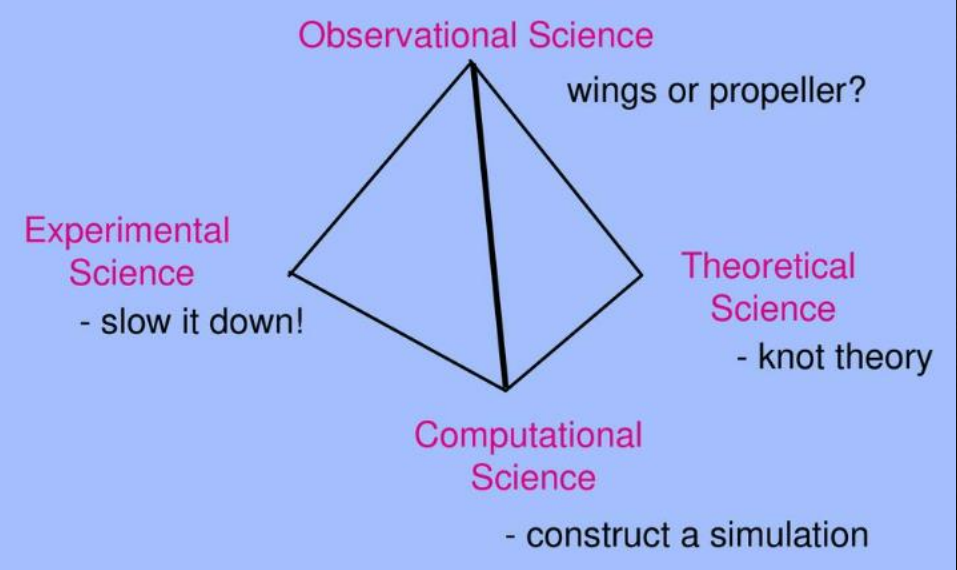
\includegraphics[width=0.8\textwidth]{images/science_four_pillars.png}
 \caption{Four Pillars of Computational Science}
 \label{fig:science_pillars}
\end{figure}

Figure~\ref{fig:science_pillars} illustrates the four complementary approaches to scientific discovery: Observational Science (observing natural phenomena), Experimental Science (controlled experiments), Theoretical Science (mathematical formulation), and Computational Science (simulation and modeling).

\subsection{The Four Pillars of Scientific Discovery}

The pyramid-shaped diagram in Figure~\ref{fig:science_pillars} represents the evolution of scientific methodology from its traditional foundations to the modern interdisciplinary approach that includes computational science. Each vertex of this pyramid represents a distinct but interconnected approach to understanding how nature behaves.

\subsubsection{Observational Science: "Wings or Propeller?"}

\begin{conceptcard}{Observational Science}
\textbf{Observational Science} involves the systematic observation and recording of natural phenomena without direct manipulation or intervention. It focuses on describing what happens in nature through careful observation and pattern recognition.
\end{conceptcard}

Observational science represents the most fundamental approach to scientific inquiry, dating back to ancient civilizations. The phrase "wings or propeller?" in the diagram captures the essence of observational science—asking questions about what we see and trying to understand the mechanisms behind observable phenomena.

\textbf{Characteristics of Observational Science:}
\begin{itemize}
    \item \textbf{Passive Data Collection}: Scientists observe and record phenomena as they naturally occur
    \item \textbf{Pattern Recognition}: Identifying trends, cycles, and relationships in observed data
    \item \textbf{Descriptive Analysis}: Cataloging and classifying natural phenomena
    \item \textbf{Hypothesis Generation}: Developing initial theories based on observations
    \item \textbf{Long-term Studies}: Monitoring changes over extended periods
\end{itemize}

\textbf{Examples of Observational Science:}
\begin{itemize}
    \item Astronomy: Observing celestial objects and cosmic phenomena
    \item Ecology: Studying animal behavior and ecosystem dynamics
    \item Meteorology: Weather pattern observation and climate monitoring
    \item Epidemiology: Disease outbreak tracking and health pattern analysis
    \item Geology: Rock formation studies and geological process observation
\end{itemize}

\subsubsection{Experimental Science: "Slow it Down!"}

\begin{conceptcard}{Experimental Science}
\textbf{Experimental Science} involves controlled manipulation of variables to test hypotheses and establish cause-and-effect relationships. The motto "slow it down!" reflects the methodical, controlled approach of experimental investigation.
\end{conceptcard}

Experimental science revolutionized our understanding of the natural world by introducing controlled conditions and systematic variable manipulation. This approach allows scientists to isolate specific factors and determine their individual effects on observed phenomena.

\textbf{Key Principles of Experimental Science:}
\begin{itemize}
    \item \textbf{Controlled Variables}: Maintaining constant conditions except for the factor being tested
    \item \textbf{Reproducibility}: Ensuring experiments can be repeated with consistent results
    \item \textbf{Isolation of Effects}: Studying one variable at a time to understand its specific impact
    \item \textbf{Statistical Analysis}: Using quantitative methods to validate results
    \item \textbf{Peer Review}: Subjecting findings to scrutiny by the scientific community
\end{itemize}

\textbf{Experimental Method Components:}
\begin{enumerate}
    \item \textbf{Hypothesis Formation}: Developing testable predictions based on observations
    \item \textbf{Experimental Design}: Planning controlled procedures to test hypotheses
    \item \textbf{Data Collection}: Gathering quantitative and qualitative measurements
    \item \textbf{Analysis and Interpretation}: Drawing conclusions from experimental results
    \item \textbf{Validation and Replication}: Confirming findings through repeated experiments
\end{enumerate}

\subsubsection{Theoretical Science: "Knot Theory"}

\begin{conceptcard}{Theoretical Science}
\textbf{Theoretical Science} involves developing mathematical models, frameworks, and abstract theories to explain natural phenomena. The reference to "knot theory" exemplifies how complex mathematical concepts can describe and predict natural behaviors.
\end{conceptcard}

Theoretical science provides the mathematical foundation for understanding natural laws and principles. It transforms observations and experimental findings into elegant mathematical formulations that can predict behavior and reveal underlying patterns.

\textbf{Components of Theoretical Science:}
\begin{itemize}
    \item \textbf{Mathematical Modeling}: Creating mathematical representations of physical phenomena
    \item \textbf{Abstract Reasoning}: Developing conceptual frameworks beyond direct observation
    \item \textbf{Predictive Capability}: Using theories to forecast future states or behaviors
    \item \textbf{Unification}: Connecting seemingly disparate phenomena under common principles
    \item \textbf{Elegance and Simplicity}: Seeking the most fundamental explanations
\end{itemize}

\textbf{Examples of Theoretical Contributions:}
\begin{itemize}
    \item Einstein's Theory of Relativity: Unified space, time, and gravity
    \item Quantum Mechanics: Mathematical description of subatomic behavior
    \item Thermodynamics: Statistical mechanics of energy and entropy
    \item Information Theory: Mathematical foundation of communication and computation
    \item Knot Theory: Mathematical study of knots with applications in DNA structure and physics
\end{itemize}

\subsubsection{Computational Science: "Construct a Simulation"}

\begin{conceptcard}{Computational Science}
\textbf{Computational Science} represents the newest pillar of scientific discovery, using computer simulations and numerical analysis to explore complex systems that are difficult to study through observation, experimentation, or pure theory alone.
\end{conceptcard}

The directive to "construct a simulation" captures the essence of computational science—creating virtual representations of real-world phenomena that can be manipulated, tested, and analyzed in ways that would be impossible with traditional approaches.

\textbf{Unique Capabilities of Computational Science:}
\begin{itemize}
    \item \textbf{Virtual Experimentation}: Conducting experiments that are impossible in reality
    \item \textbf{Scale Bridging}: Connecting phenomena across vastly different spatial and temporal scales
    \item \textbf{Parameter Exploration}: Testing thousands of scenarios rapidly and systematically
    \item \textbf{Visualization}: Making invisible phenomena visible and understandable
    \item \textbf{Prediction}: Forecasting future states based on current conditions and known laws
\end{itemize}

\textbf{Computational Approaches:}
\begin{enumerate}
    \item \textbf{Numerical Simulation}: Solving mathematical models computationally
    \item \textbf{Data Analysis}: Processing large datasets to extract patterns and insights
    \item \textbf{Machine Learning}: Using algorithms to identify patterns and make predictions
    \item \textbf{Visualization}: Creating graphical representations of complex data and phenomena
    \item \textbf{Optimization}: Finding optimal solutions to complex problems
\end{enumerate}

\subsection{The Synergistic Diamond: Integrating Four Approaches}

The diamond configuration in Figure~\ref{fig:science_pillars} is not merely a geometric arrangement—it represents the interconnected and complementary nature of these four scientific approaches. Each pillar contributes unique strengths while addressing the limitations of the others:

\begin{itemize}
    \item \textbf{Observational-Experimental Synergy}: Observations guide experimental design, while experiments validate or refute observational hypotheses
    \item \textbf{Theoretical-Computational Integration}: Theories provide the mathematical foundation for simulations, while computational results test theoretical predictions
    \item \textbf{Cross-Pillar Validation}: Findings from one approach can be validated through methods from other pillars
    \item \textbf{Complementary Perspectives}: Each approach reveals different aspects of the same natural phenomena
\end{itemize}

\begin{highlightbox}{The Power of Integration}
Modern scientific breakthroughs increasingly emerge from the integration of all four approaches:
\begin{itemize}
    \item \textbf{Climate Science}: Combines observational data, laboratory experiments, theoretical models, and computational simulations
    \item \textbf{Drug Discovery}: Integrates biological observations, controlled experiments, theoretical chemistry, and computational molecular modeling
    \item \textbf{Astrophysics}: Merges telescopic observations, laboratory plasma experiments, theoretical physics, and numerical cosmological simulations
    \item \textbf{Materials Science}: Unifies structural observations, experimental testing, theoretical solid-state physics, and computational materials design
\end{itemize}
\end{highlightbox}

\subsection{The Tripartite Nature of Computational Science}

One of the most significant aspects of computational science is its tripartite structure, which integrates three essential components into a cohesive methodology. This approach distinguishes computational science from other computational fields and establishes it as a unique scientific discipline.

\begin{conceptcard}{The Tripartite Foundation}
The \textbf{Tripartite Approach} to computational science recognizes that effective computational research requires the seamless integration of three fundamental pillars: \textbf{Architecture} (Computing Environment), \textbf{Algorithm} (Mathematical Model), and \textbf{Application} (Science). These three components work synergistically to create computational models that bridge theory and practice.
\end{conceptcard}

\subsection{Understanding the Tripartite Triangle}

\begin{figure}[h]
 \centering
 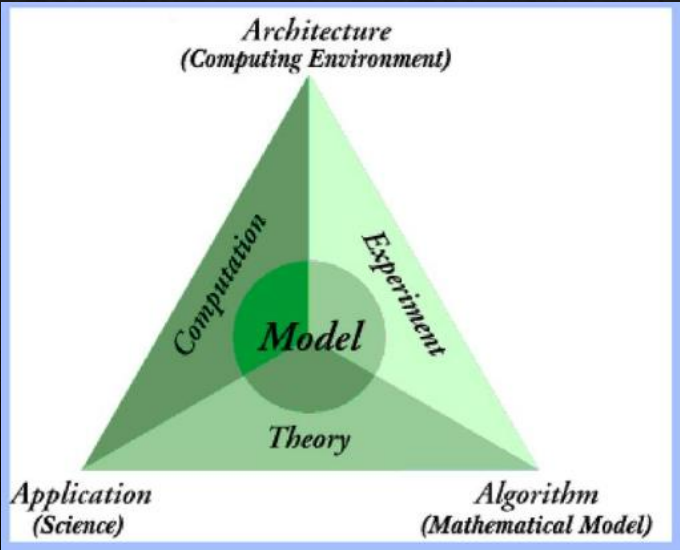
\includegraphics[width=0.7\textwidth]{images/tripartite_triangle.png}
 \caption{Tripartite Approach to Computational Science}
 \label{fig:tripartite_approach}
\end{figure}

Figure~\ref{fig:tripartite_approach} illustrates the tripartite approach as a triangle with three vertices representing the fundamental components of computational science. This geometric representation is not merely symbolic—it reflects the inherent interdependence and balance required among these components for successful computational science endeavors.

The triangle's structure emphasizes several key principles:

\begin{itemize}
    \item \textbf{Equality of Importance}: Each vertex represents an equally crucial component; weakness in any one area compromises the entire endeavor
    \item \textbf{Interconnectedness}: The edges of the triangle represent the critical interfaces between components
    \item \textbf{Central Integration}: The model at the center emerges from the synthesis of all three components
    \item \textbf{Dynamic Balance}: Success requires maintaining balance among all three aspects throughout the research process
\end{itemize}

\subsubsection{Vertex 1: Architecture (Computing Environment)}

\begin{conceptcard}{Architecture - The Computing Foundation}
\textbf{Architecture} encompasses the entire computational infrastructure that enables scientific computing, from hardware platforms and software frameworks to programming paradigms and system design principles. It represents the "how" of computational implementation.
\end{conceptcard}

The Architecture vertex addresses the fundamental computational infrastructure questions that determine what is computationally feasible and how efficiently it can be accomplished.

\textbf{Hardware Architecture Components:}
\begin{itemize}
    \item \textbf{Processing Units}: CPUs, GPUs, specialized processors (FPGAs, TPUs)
    \item \textbf{Memory Hierarchy}: RAM, cache systems, storage architectures
    \item \textbf{Network Infrastructure}: High-speed interconnects, distributed computing networks
    \item \textbf{Parallel Computing Platforms}: Shared memory, distributed memory, hybrid systems
    \item \textbf{Accelerator Technologies}: Graphics cards, quantum processors, neuromorphic chips
\end{itemize}

\textbf{Software Architecture Elements:}
\begin{itemize}
    \item \textbf{Programming Languages}: Python, C/C++, Fortran, Julia, R, MATLAB
    \item \textbf{Development Frameworks}: Scientific computing libraries, parallel programming models
    \item \textbf{Runtime Systems}: Operating systems, job schedulers, resource managers
    \item \textbf{Development Tools}: Compilers, debuggers, profilers, version control systems
    \item \textbf{Middleware}: Database systems, visualization tools, workflow management
\end{itemize}

\textbf{Computational Paradigms:}
\begin{itemize}
    \item \textbf{High-Performance Computing}: Supercomputing, cluster computing
    \item \textbf{Cloud Computing}: On-demand resources, scalable infrastructure
    \item \textbf{Edge Computing}: Distributed processing, real-time computation
    \item \textbf{Grid Computing}: Resource sharing across institutions
    \item \textbf{Quantum Computing}: Quantum algorithms, quantum simulators
\end{itemize}

\textbf{Architecture Considerations:}
\begin{itemize}
    \item \textbf{Performance Optimization}: Maximizing computational throughput and minimizing execution time
    \item \textbf{Scalability}: Handling increasing problem sizes and computational demands
    \item \textbf{Resource Efficiency}: Optimal utilization of computational resources
    \item \textbf{Reliability}: Ensuring system stability and fault tolerance
    \item \textbf{Accessibility}: Making computational resources available to researchers
\end{itemize}

\subsubsection{Vertex 2: Algorithm (Mathematical Model)}

\begin{conceptcard}{Algorithm - The Mathematical Foundation}
\textbf{Algorithm} represents the mathematical and computational methods that transform real-world problems into solvable computational forms. It encompasses both the mathematical modeling of phenomena and the algorithmic approaches for solving the resulting equations.
\end{conceptcard}

The Algorithm vertex bridges the gap between abstract mathematical descriptions of natural phenomena and concrete computational procedures that can be executed on computing systems.

\textbf{Mathematical Modeling Components:}
\begin{itemize}
    \item \textbf{Differential Equations}: Ordinary and partial differential equations describing dynamic systems
    \item \textbf{Statistical Models}: Probabilistic descriptions of uncertain phenomena
    \item \textbf{Optimization Models}: Mathematical formulations of decision problems
    \item \textbf{Discrete Models}: Graph theory, combinatorial optimization, cellular automata
    \item \textbf{Stochastic Models}: Random processes, Monte Carlo methods, uncertainty quantification
\end{itemize}

\textbf{Numerical Methods:}
\begin{itemize}
    \item \textbf{Numerical Integration}: Euler methods, Runge-Kutta schemes, multistep methods
    \item \textbf{Linear Algebra}: Matrix operations, eigenvalue problems, iterative solvers
    \item \textbf{Finite Element Methods}: Spatial discretization for partial differential equations
    \item \textbf{Finite Difference Methods}: Grid-based approximations of derivatives
    \item \textbf{Spectral Methods}: Fourier and polynomial-based solution techniques
\end{itemize}

\textbf{Algorithmic Design Principles:}
\begin{itemize}
    \item \textbf{Accuracy}: Ensuring numerical solutions accurately represent the mathematical model
    \item \textbf{Stability}: Maintaining solution reliability over long computational runs
    \item \textbf{Efficiency}: Minimizing computational complexity and resource requirements
    \item \textbf{Robustness}: Handling edge cases and numerical difficulties gracefully
    \item \textbf{Parallelizability}: Designing algorithms suitable for parallel execution
\end{itemize}

\textbf{Error Analysis and Control:}
\begin{itemize}
    \item \textbf{Discretization Error}: Errors from approximating continuous problems
    \item \textbf{Round-off Error}: Accumulation of floating-point arithmetic errors
    \item \textbf{Convergence Analysis}: Theoretical guarantees for algorithm behavior
    \item \textbf{Adaptive Methods}: Dynamic adjustment of computational parameters
    \item \textbf{Uncertainty Quantification}: Propagation of input uncertainties through calculations
\end{itemize}

\subsubsection{Vertex 3: Application (Science)}

\begin{conceptcard}{Application - The Scientific Foundation}
\textbf{Application} represents the domain-specific scientific knowledge, understanding, and expertise that drives computational science research. It encompasses the scientific questions, physical understanding, and validation criteria that give meaning and context to computational investigations.
\end{conceptcard}

The Application vertex ensures that computational science serves real scientific purposes and produces meaningful, interpretable, and actionable results within specific scientific domains.

\textbf{Domain-Specific Knowledge:}
\begin{itemize}
    \item \textbf{Physical Sciences}: Physics, chemistry, astronomy, materials science
    \item \textbf{Life Sciences}: Biology, medicine, ecology, bioinformatics
    \item \textbf{Earth Sciences}: Climatology, geology, oceanography, atmospheric science
    \item \textbf{Engineering}: Mechanical, electrical, aerospace, civil engineering
    \item \textbf{Social Sciences}: Economics, sociology, political science, psychology
\end{itemize}

\textbf{Scientific Methodology:}
\begin{itemize}
    \item \textbf{Problem Formulation}: Translating scientific questions into computational problems
    \item \textbf{Hypothesis Development}: Creating testable predictions from computational models
    \item \textbf{Experimental Design}: Planning computational experiments and parameter studies
    \item \textbf{Data Analysis}: Interpreting computational results in scientific context
    \item \textbf{Validation Studies}: Comparing computational predictions with empirical data
\end{itemize}

\textbf{Scientific Understanding Requirements:}
\begin{itemize}
    \item \textbf{Fundamental Principles}: Deep understanding of governing physical laws and relationships
    \item \textbf{Phenomenological Knowledge}: Awareness of relevant phenomena and their characteristics
    \item \textbf{Scale Considerations}: Understanding of relevant temporal and spatial scales
    \item \textbf{Limiting Cases}: Knowledge of simplified scenarios and analytical solutions
    \item \textbf{Physical Intuition}: Ability to assess whether computational results are reasonable
\end{itemize}

\textbf{Validation and Verification:}
\begin{itemize}
    \item \textbf{Model Validation}: Ensuring models accurately represent real-world phenomena
    \item \textbf{Experimental Comparison}: Benchmarking against laboratory and field measurements
    \item \textbf{Cross-Validation}: Comparing different computational approaches
    \item \textbf{Sensitivity Analysis}: Understanding model response to parameter variations
    \item \textbf{Uncertainty Assessment}: Quantifying confidence in computational predictions
\end{itemize}

\subsubsection{The Central Model: Synthesis and Integration}

\begin{conceptcard}{The Computational Model}
The \textbf{Model} at the center of the tripartite triangle represents the integrated computational representation that emerges from the synthesis of Architecture, Algorithm, and Application. It is the concrete manifestation of computational science that enables scientific discovery and understanding.
\end{conceptcard}

The central model is not simply the sum of its three components—it represents a new entity that emerges from their integration and interaction. This model embodies the unique value proposition of computational science: the ability to explore, predict, and understand complex phenomena through computational means.

\textbf{Model Characteristics:}
\begin{itemize}
    \item \textbf{Computational Representation}: Digital encoding of scientific phenomena
    \item \textbf{Predictive Capability}: Ability to forecast future states or behaviors
    \item \textbf{Exploratory Power}: Capacity to investigate scenarios impossible in reality
    \item \textbf{Scalable Complexity}: Capability to handle problems across different scales
    \item \textbf{Interactive Analysis}: Real-time exploration and parameter manipulation
\end{itemize}

\textbf{Model Functions:}
\begin{itemize}
    \item \textbf{Virtual Experimentation}: Conducting experiments in computational space
    \item \textbf{Hypothesis Testing}: Evaluating scientific theories and predictions
    \item \textbf{Parameter Space Exploration}: Systematic investigation of model behaviors
    \item \textbf{Optimization}: Finding optimal designs or operating conditions
    \item \textbf{Sensitivity Analysis}: Understanding factor importance and model robustness
\end{itemize}

\subsection{The Synergistic Relationships: Triangle Edges}

The edges of the tripartite triangle represent the critical interfaces and relationships between the three fundamental components. These relationships are bidirectional and essential for successful computational science.

\subsubsection{Architecture-Algorithm Interface}

The relationship between Architecture and Algorithm involves the optimization of computational methods for specific hardware platforms and the design of algorithms that can effectively utilize available computational resources.

\textbf{Key Considerations:}
\begin{itemize}
    \item \textbf{Algorithm-Hardware Matching}: Choosing algorithms suited to available computational architectures
    \item \textbf{Performance Optimization}: Tuning algorithms for specific hardware characteristics
    \item \textbf{Parallel Algorithm Design}: Developing algorithms that can exploit parallel processing capabilities
    \item \textbf{Memory Management}: Optimizing data access patterns for hierarchical memory systems
    \item \textbf{Scalability Planning}: Ensuring algorithms can utilize larger computational resources effectively
\end{itemize}

\subsubsection{Algorithm-Application Interface}

The Algorithm-Application interface focuses on ensuring that mathematical models and computational methods accurately capture the essential physics and behavior of the scientific system under study.

\textbf{Key Considerations:}
\begin{itemize}
    \item \textbf{Physical Fidelity}: Ensuring mathematical models represent relevant physics
    \item \textbf{Approximation Assessment}: Understanding the impact of mathematical simplifications
    \item \textbf{Scale Matching}: Choosing mathematical approaches appropriate for the relevant scales
    \item \textbf{Validation Requirements}: Designing computational methods that can be validated against data
    \item \textbf{Scientific Interpretation}: Ensuring computational results can be interpreted scientifically
\end{itemize}

\subsubsection{Application-Architecture Interface}

The Application-Architecture relationship involves understanding how scientific requirements drive computational resource needs and how computational limitations constrain scientific investigations.

\textbf{Key Considerations:}
\begin{itemize}
    \item \textbf{Resource Requirements}: Estimating computational needs for scientific problems
    \item \textbf{Constraint Recognition}: Understanding how computational limitations affect scientific scope
    \item \textbf{Technology Selection}: Choosing appropriate computational tools for scientific applications
    \item \textbf{Collaboration Models}: Organizing computational resources for scientific research
    \item \textbf{Future Planning}: Anticipating computational needs for advancing scientific understanding
\end{itemize}

\subsection{Practical Implementation of the Tripartite Approach}

\begin{examplebox}{Tripartite Approach in Climate Modeling}
Consider a climate modeling project that exemplifies the tripartite approach:

\textbf{Application (Science):}
\begin{itemize}
    \item Understanding atmospheric and oceanic physics
    \item Knowledge of climate system interactions
    \item Validation against observational climate data
    \item Scientific questions about climate change impacts
\end{itemize}

\textbf{Algorithm (Mathematical Model):}
\begin{itemize}
    \item Navier-Stokes equations for fluid dynamics
    \item Radiative transfer equations for energy balance
    \item Numerical methods for partial differential equations
    \item Grid-based discretization of Earth's surface
\end{itemize}

\textbf{Architecture (Computing Environment):}
\begin{itemize}
    \item High-performance computing clusters
    \item Parallel programming with MPI
    \item Fortran and C++ implementation
    \item Distributed data storage systems
\end{itemize}

\textbf{Integrated Model:}
The resulting global climate model can simulate Earth's climate system, predict future climate scenarios, and explore the impacts of different emission pathways, demonstrating how the three components work together to enable scientific discovery.
\end{examplebox}

\subsection{Benefits of the Tripartite Approach}

The tripartite framework provides several important benefits for computational science practice:

\begin{itemize}
    \item \textbf{Systematic Planning}: Ensures all essential components are considered in project design
    \item \textbf{Balanced Development}: Prevents overemphasis on any single aspect at the expense of others
    \item \textbf{Quality Assurance}: Provides checkpoints for evaluating project progress and success
    \item \textbf{Interdisciplinary Communication}: Offers a common framework for collaboration across disciplines
    \item \textbf{Educational Structure}: Organizes computational science curriculum and training
    \item \textbf{Research Evaluation}: Provides criteria for assessing computational science contributions
\end{itemize}

\subsection{Challenges in Tripartite Integration}

While the tripartite approach provides a powerful framework, implementing it effectively presents several challenges:

\begin{itemize}
    \item \textbf{Expertise Requirements}: Few individuals possess deep knowledge in all three areas
    \item \textbf{Communication Barriers}: Different communities use different languages and approaches
    \item \textbf{Resource Allocation}: Balancing investment across the three components
    \item \textbf{Timeline Coordination}: Synchronizing development across different aspects
    \item \textbf{Quality Control}: Maintaining standards across diverse technical areas
    \item \textbf{Technology Evolution}: Keeping pace with rapid changes in all three domains
\end{itemize}

The tripartite nature of computational science thus represents both the strength and the challenge of the field—its power comes from integration across disciplines, but this integration requires careful attention to all three fundamental components and their interactions.

\subsection{The Interdisciplinary Venn Diagram Perspective}

\begin{figure}[h]
 \centering
 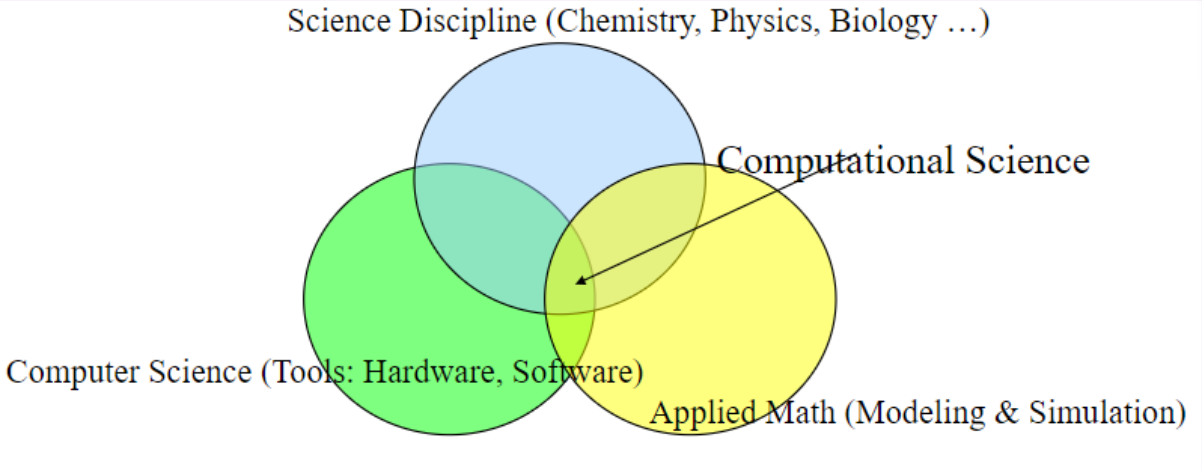
\includegraphics[width=0.8\textwidth]{images/computational_science_venn.png}
 \caption{Computational Science at the Intersection of Disciplines}
 \label{fig:computational_science_venn}
\end{figure}

Figure~\ref{fig:computational_science_venn} provides another perspective on computational science, illustrating its position at the intersection of three major academic disciplines: Science, Computer Science, and Applied Mathematics.

Another way to understand computational science is through its position at the intersection of three major academic disciplines. This Venn diagram perspective illustrates how computational science draws from and contributes to:

\begin{itemize}
  \item \textbf{Science Disciplines} (Chemistry, Physics, Biology, Economics, etc.): Providing the domain knowledge, scientific questions, and validation criteria
  \item \textbf{Computer Science}: Contributing algorithms, data structures, software engineering practices, and computational thinking methodologies
  \item \textbf{Applied Mathematics}: Offering mathematical modeling techniques, numerical analysis, optimization methods, and statistical approaches
\end{itemize}

This interdisciplinary nature means that computational scientists must develop competencies across multiple fields, making them uniquely positioned to tackle complex, multi-faceted problems that cannot be adequately addressed within the boundaries of a single discipline.

\subsection{The Three Pillars of Science}

Modern science rests on three fundamental pillars, each offering unique perspectives and methodologies for understanding the natural world:

\begin{enumerate}
  \item \textbf{Theory (Theoretical Science)}: Mathematical models and theoretical frameworks that describe natural phenomena through equations, principles, and abstract reasoning. Theoretical science seeks to understand the fundamental laws governing natural processes and provides the mathematical foundation for scientific understanding. Examples include Einstein's theory of relativity, quantum mechanics, and thermodynamic principles.
      
  \item \textbf{Experiment (Experimental Science)}: Empirical observations and laboratory investigations that test hypotheses and gather data about the real world. Experimental science involves controlled manipulation of variables to isolate cause-and-effect relationships and validate theoretical predictions. Examples include laboratory experiments, field studies, and clinical trials.
      
  \item \textbf{Computation (Computational Science)}: Computer simulations and numerical analysis that enable exploration of complex systems through mathematical modeling and algorithmic processing. Computational science allows scientists to investigate phenomena that are inaccessible through experimentation alone and to test theoretical predictions under various conditions.
\end{enumerate}

Each pillar has its unique strengths and limitations:

\begin{itemize}
  \item \textbf{Theory} provides elegant mathematical descriptions but may involve simplifying assumptions that limit applicability to real-world systems
  \item \textbf{Experiment} offers direct contact with reality but may be constrained by practical limitations, safety concerns, or ethical considerations
  \item \textbf{Computation} enables exploration of complex scenarios but depends on the accuracy of underlying models and algorithms
\end{itemize}

The power of modern science lies in the synergistic combination of all three pillars, where computational science serves as a bridge between theoretical predictions and experimental observations.

\begin{highlightbox}{Why Computational Science Matters}
Computational science has become essential because:
\begin{itemize}
  \item \textbf{Scale Limitations}: Many phenomena occur at scales (astronomical, molecular, geological time) that are difficult or impossible to observe directly
  \item \textbf{Complexity}: Real-world systems often involve multiple interacting components that cannot be understood through simple theoretical models
  \item \textbf{Safety and Ethics}: Some experiments are too dangerous, destructive, or ethically problematic to perform (nuclear explosions, pandemic spread, ecological disasters)
  \item \textbf{Cost and Time}: Computational experiments can explore thousands of scenarios quickly and inexpensively compared to physical experiments
  \item \textbf{Accessibility}: Simulations can make phenomena visible and understandable in ways that enhance scientific education and public understanding
  \item \textbf{Prediction and Design}: Computational models enable prediction of future states and optimization of design parameters before physical implementation
\end{itemize}
\end{highlightbox}

\section{Characteristics of Computational Science}

\subsection{Interdisciplinary Nature}

Computational science is fundamentally interdisciplinary, requiring the integration of knowledge and methods from multiple fields. This interdisciplinary nature is not merely a characteristic but a necessity, as computational science problems typically span traditional academic boundaries and require expertise from diverse domains.

The main contributing disciplines include:

\begin{itemize}
  \item \textbf{Computer Science}: Provides the computational foundation including:
  \begin{itemize}
    \item Algorithms and data structures for efficient problem-solving
    \item Software engineering practices for reliable and maintainable code
    \item High-performance computing techniques for large-scale simulations
    \item Database management for handling large datasets
    \item Human-computer interaction for effective visualization and user interfaces
  \end{itemize}
      
  \item \textbf{Mathematics and Applied Mathematics}: Offers the analytical framework through:
  \begin{itemize}
    \item Numerical analysis for approximating solutions to mathematical problems
    \item Statistics and probability for uncertainty quantification and data analysis
    \item Discrete mathematics for algorithmic thinking and optimization
    \item Calculus and differential equations for modeling continuous phenomena
    \item Linear algebra for efficient computation and data representation
  \end{itemize}
      
  \item \textbf{Domain Sciences}: Provide the scientific context and validation criteria:
  \begin{itemize}
    \item Physics: Fundamental laws and principles governing natural phenomena
    \item Chemistry: Molecular interactions and chemical processes
    \item Biology: Life processes, evolution, and ecological systems
    \item Engineering: Design principles, optimization, and practical constraints
    \item Economics: Market behavior, decision-making, and resource allocation
    \item Social Sciences: Human behavior, social networks, and cultural dynamics
  \end{itemize}
      
  \item \textbf{Applied Mathematics and Scientific Computing}: Bridge the gap between pure mathematics and practical computation:
  \begin{itemize}
    \item Mathematical modeling techniques for translating real-world problems into mathematical representations
    \item Optimization methods for finding optimal solutions under constraints
    \item Differential equations for modeling change and dynamics
    \item Scientific visualization for understanding and communicating results
  \end{itemize}
\end{itemize}

This interdisciplinary nature creates both opportunities and challenges. While it enables the solution of complex, real-world problems, it also requires computational scientists to develop broad competencies and effective communication skills across disciplines.

\subsection{Problem-Solving Approach}

Computational science employs a systematic, methodical approach to problem-solving that distinguishes it from ad-hoc programming or purely theoretical analysis. This approach ensures reproducibility, reliability, and scientific rigor in computational research.

The computational science problem-solving methodology involves six interconnected phases:

\begin{enumerate}
  \item \textbf{Problem Identification and Formulation}: 
  \begin{itemize}
    \item Clearly defining the scientific or engineering problem
    \item Identifying the key questions that need to be answered
    \item Determining the scope and boundaries of the investigation
    \item Establishing success criteria and performance metrics
    \item Assessing available resources and constraints
  \end{itemize}
      
  \item \textbf{Mathematical Modeling and Abstraction}: 
  \begin{itemize}
    \item Creating mathematical representations of the physical, biological, or social system
    \item Identifying relevant variables, parameters, and relationships
    \item Making appropriate assumptions and simplifications
    \item Selecting suitable mathematical frameworks (differential equations, statistical models, etc.)
    \item Validating the conceptual model against domain knowledge
  \end{itemize}
      
  \item \textbf{Algorithm Development and Computational Design}: 
  \begin{itemize}
    \item Designing computational methods to solve the mathematical model
    \item Selecting appropriate numerical algorithms and techniques
    \item Considering computational complexity and efficiency
    \item Planning for scalability and parallel processing when necessary
    \item Designing data structures for efficient storage and access
  \end{itemize}
      
  \item \textbf{Implementation and Programming}: 
  \begin{itemize}
    \item Programming the solution using appropriate tools and languages
    \item Following software engineering best practices
    \item Implementing error handling and input validation
    \item Creating modular, reusable, and maintainable code
    \item Documenting the implementation for reproducibility
  \end{itemize}
      
  \item \textbf{Simulation, Execution, and Analysis}: 
  \begin{itemize}
    \item Running computations with appropriate parameters and initial conditions
    \item Monitoring performance and resource utilization
    \item Collecting and organizing computational results
    \item Performing statistical analysis and uncertainty quantification
    \item Visualizing results for interpretation and communication
  \end{itemize}
      
  \item \textbf{Validation, Verification, and Interpretation}: 
  \begin{itemize}
    \item Ensuring the model and implementation are correct and reliable
    \item Comparing results with experimental data, analytical solutions, or benchmarks
    \item Assessing the accuracy and limitations of the computational approach
    \item Interpreting results in the context of the original scientific question
    \item Drawing conclusions and identifying areas for future research
  \end{itemize}
\end{enumerate}

This systematic approach ensures that computational science projects are conducted with scientific rigor and that results are reliable, reproducible, and meaningful within their domain of application.

\section{Computational Thinking}

\begin{conceptcard}{Computational Thinking}
\textbf{Computational Thinking} is a problem-solving methodology that involves breaking down complex problems into manageable components and developing step-by-step solutions that can be implemented computationally. It represents a fundamental approach to understanding and solving problems that combines mathematical reasoning, logical thinking, and systematic analysis.
\end{conceptcard}

Computational thinking is not limited to computer science or computational science—it is a general problem-solving approach that can be applied across all disciplines. It provides a systematic way to approach complex problems by leveraging the same strategies that make computer algorithms effective: decomposition, pattern recognition, abstraction, and systematic solution design.

The importance of computational thinking in the modern world cannot be overstated. As our society becomes increasingly digital and data-driven, the ability to think computationally becomes a fundamental literacy skill, comparable to reading, writing, and arithmetic. Computational thinking helps us understand how to approach problems systematically, design efficient solutions, and communicate complex ideas clearly.

\subsection{Key Components of Computational Thinking}

Computational thinking comprises four fundamental components that work together to provide a comprehensive problem-solving framework:

\begin{enumerate}
  \item \textbf{Decomposition}: Breaking complex problems into smaller, more manageable sub-problems
  \begin{itemize}
    \item Identifying the main components of a complex system
    \item Dividing large problems into smaller, solvable pieces
    \item Creating hierarchical structures that organize problem components
    \item Enabling parallel work on different aspects of the problem
    \item Making complex problems less overwhelming and more approachable
  \end{itemize}
      
  \item \textbf{Pattern Recognition}: Identifying similarities, trends, and regularities in data or problems
  \begin{itemize}
    \item Recognizing recurring themes or structures across different contexts
    \item Identifying relationships between variables or components
    \item Finding commonalities that can be exploited for efficient solutions
    \item Detecting anomalies or deviations from expected patterns
    \item Using patterns to predict future behavior or outcomes
  \end{itemize}
      
  \item \textbf{Abstraction}: Focusing on essential features while ignoring irrelevant details
  \begin{itemize}
    \item Identifying the core aspects of a problem that are crucial for solution
    \item Creating simplified models that capture essential behavior
    \item Hiding complexity behind well-defined interfaces
    \item Generalizing specific solutions to broader classes of problems
    \item Developing reusable components and frameworks
  \end{itemize}
      
  \item \textbf{Algorithm Design}: Creating step-by-step procedures to solve problems
  \begin{itemize}
    \item Developing systematic, logical sequences of operations
    \item Ensuring procedures are clear, unambiguous, and complete
    \item Optimizing for efficiency and effectiveness
    \item Considering edge cases and error conditions
    \item Designing solutions that can be implemented and executed reliably
  \end{itemize}
\end{enumerate}

\subsection{Computational Thinking in Practice}

\begin{examplebox}{Computational Thinking in Weather Prediction}
Consider the complex problem of predicting weather patterns:

\textbf{Decomposition:} Break the atmosphere into smaller components:
\begin{itemize}
  \item Atmospheric pressure systems
  \item Temperature distributions
  \item Humidity and moisture content
  \item Wind patterns and air circulation
  \item Solar radiation and heat transfer
  \item Geographical features and their effects
\end{itemize}

\textbf{Pattern Recognition:} Identify recurring meteorological phenomena:
\begin{itemize}
  \item Seasonal weather cycles and climate patterns
  \item Pressure system movements and interactions
  \item Temperature gradients and their effects on wind
  \item Historical weather data and statistical trends
  \item Relationships between different atmospheric variables
\end{itemize}

\textbf{Abstraction:} Focus on essential atmospheric variables:
\begin{itemize}
  \item Use key meteorological variables while ignoring minor fluctuations
  \item Create simplified models of atmospheric physics
  \item Develop mathematical representations of weather systems
  \item Abstract complex interactions into manageable equations
\end{itemize}

\textbf{Algorithm Design:} Develop numerical methods for weather simulation:
\begin{itemize}
  \item Create algorithms to solve atmospheric equations numerically
  \item Design procedures for data assimilation and model initialization
  \item Develop methods for uncertainty quantification and ensemble forecasting
  \item Implement efficient computational strategies for real-time prediction
\end{itemize}
\end{examplebox}

\subsection{Benefits of Computational Thinking}

Computational thinking provides numerous advantages for problem-solving across disciplines:

\begin{itemize}
  \item \textbf{Systematic Approach}: Provides a structured methodology for tackling complex problems
  \item \textbf{Scalability}: Solutions can be extended to handle larger or more complex instances
  \item \textbf{Reusability}: Components and strategies can be applied to similar problems
  \item \textbf{Clarity}: Forces clear thinking about problem structure and solution strategies
  \item \textbf{Efficiency}: Helps identify the most effective approaches and avoid unnecessary complexity
  \item \textbf{Communication}: Provides a common framework for describing problems and solutions
  \item \textbf{Automation}: Enables the development of solutions that can be implemented computationally
\end{itemize}

\subsection{Computational Thinking Beyond Computer Science}

While computational thinking is fundamental to computational science, its applications extend far beyond technical fields:

\begin{itemize}
  \item \textbf{Education}: Organizing curriculum, breaking down learning objectives, designing assessments
  \item \textbf{Business}: Process optimization, strategic planning, resource allocation
  \item \textbf{Healthcare}: Diagnosis procedures, treatment protocols, epidemiological studies
  \item \textbf{Social Sciences}: Survey design, data collection strategies, policy analysis
  \item \textbf{Arts and Humanities}: Digital humanities projects, creative coding, interactive media
\end{itemize}

\section{Applications of Computational Science}

Computational science has revolutionized numerous fields:

\subsection{Physical Sciences}
\begin{itemize}
  \item \textbf{Climate Modeling}: Global climate simulations and weather prediction
  \item \textbf{Astrophysics}: Galaxy formation, black hole simulations, cosmological models
  \item \textbf{Materials Science}: Molecular dynamics, crystal structure prediction
  \item \textbf{Quantum Mechanics}: Electronic structure calculations, quantum simulations
\end{itemize}

\subsection{Life Sciences}
\begin{itemize}
  \item \textbf{Bioinformatics}: Genome analysis, protein folding, phylogenetic trees
  \item \textbf{Epidemiology}: Disease spread modeling, pandemic prediction
  \item \textbf{Drug Discovery}: Molecular docking, drug-target interactions
  \item \textbf{Systems Biology}: Metabolic networks, gene regulatory networks
\end{itemize}

\subsection{Engineering and Technology}
\begin{itemize}
  \item \textbf{Aerospace Engineering}: Flight simulations, spacecraft design
  \item \textbf{Civil Engineering}: Structural analysis, earthquake modeling
  \item \textbf{Computer Graphics}: Animation, visual effects, virtual reality
  \item \textbf{Robotics}: Path planning, control systems, machine learning
\end{itemize}

\subsection{Social Sciences and Economics}
\begin{itemize}
  \item \textbf{Economics}: Market modeling, risk analysis, algorithmic trading
  \item \textbf{Political Science}: Election prediction, policy analysis
  \item \textbf{Sociology}: Social network analysis, urban planning
  \item \textbf{Psychology}: Cognitive modeling, behavioral simulations
\end{itemize}

\section{Types of Computational Models}

\subsection{Mathematical Models}
\begin{itemize}
  \item \textbf{Differential Equations}: Continuous change models (population growth, heat transfer)
  \item \textbf{Discrete Models}: Step-by-step evolution (cellular automata, agent-based models)
  \item \textbf{Statistical Models}: Probabilistic relationships (regression, machine learning)
  \item \textbf{Network Models}: Graph-based representations (social networks, transportation)
\end{itemize}

\subsection{Computational Approaches}
\begin{itemize}
  \item \textbf{Deterministic Simulations}: Predictable outcomes based on initial conditions
  \item \textbf{Stochastic Simulations}: Incorporating randomness and uncertainty
  \item \textbf{Monte Carlo Methods}: Random sampling for complex integrations
  \item \textbf{Machine Learning}: Data-driven pattern recognition and prediction
\end{itemize}

\section{The Computational Science Workflow}

\begin{conceptcard}{Computational Science Methodology}
The computational science workflow follows a systematic approach that ensures reliable and reproducible results.
\end{conceptcard}

\subsection{Phase 1: Problem Formulation}
\begin{enumerate}
  \item Identify the scientific question or engineering problem
  \item Define objectives and success criteria
  \item Gather relevant background knowledge
  \item Determine available resources and constraints
\end{enumerate}

\subsection{Phase 2: Mathematical Modeling}
\begin{enumerate}
  \item Choose appropriate mathematical frameworks
  \item Define variables, parameters, and relationships
  \item Make necessary assumptions and approximations
  \item Validate the mathematical model conceptually
\end{enumerate}

\subsection{Phase 3: Computational Implementation}
\begin{enumerate}
  \item Select appropriate algorithms and numerical methods
  \item Choose programming languages and computational tools
  \item Implement the model in code
  \item Test and debug the implementation
\end{enumerate}

\subsection{Phase 4: Simulation and Analysis}
\begin{enumerate}
  \item Design computational experiments
  \item Run simulations with various parameters
  \item Collect and organize results
  \item Perform statistical analysis of outputs
\end{enumerate}

\subsection{Phase 5: Validation and Verification}
\begin{enumerate}
  \item \textbf{Verification}: Ensure the code correctly implements the mathematical model
  \item \textbf{Validation}: Confirm the model accurately represents the real system
  \item Compare results with experimental data or known solutions
  \item Assess uncertainty and error bounds
\end{enumerate}

\subsection{Phase 6: Interpretation and Communication}
\begin{enumerate}
  \item Interpret results in the context of the original problem
  \item Draw scientific conclusions and insights
  \item Communicate findings to stakeholders
  \item Document methodology for reproducibility
\end{enumerate}

\section{Tools and Technologies}

\subsection{Programming Languages}
\begin{itemize}
  \item \textbf{Python}: Data science, scientific computing, machine learning
  \item \textbf{R}: Statistical analysis, data visualization
  \item \textbf{MATLAB}: Numerical computing, engineering applications
  \item \textbf{C/C++}: High-performance computing, system programming
  \item \textbf{Julia}: High-performance scientific computing
  \item \textbf{Fortran}: Traditional scientific computing, numerical libraries
\end{itemize}

\subsection{Computational Platforms}
\begin{itemize}
  \item \textbf{High-Performance Computing (HPC)}: Supercomputers, parallel processing
  \item \textbf{Cloud Computing}: Scalable, on-demand computational resources
  \item \textbf{Grid Computing}: Distributed computing across networks
  \item \textbf{GPU Computing}: Graphics processing units for parallel computation
\end{itemize}

\subsection{Software Libraries and Frameworks}
\begin{itemize}
  \item \textbf{Scientific Libraries}: NumPy, SciPy, Pandas (Python), GSL (C++)
  \item \textbf{Visualization Tools}: Matplotlib, Plotly, Paraview, Gnuplot
  \item \textbf{Machine Learning}: TensorFlow, PyTorch, Scikit-learn
  \item \textbf{Simulation Frameworks}: OpenFOAM, COMSOL, ANSYS
\end{itemize}

\section{Challenges in Computational Science}

\subsection{Technical Challenges}
\begin{itemize}
  \item \textbf{Scalability}: Handling increasingly large datasets and complex models
  \item \textbf{Accuracy}: Balancing computational efficiency with numerical precision
  \item \textbf{Uncertainty Quantification}: Managing and propagating uncertainties
  \item \textbf{Verification and Validation}: Ensuring model reliability and accuracy
\end{itemize}

\subsection{Methodological Challenges}
\begin{itemize}
  \item \textbf{Model Selection}: Choosing appropriate models for specific problems
  \item \textbf{Parameter Estimation}: Determining model parameters from limited data
  \item \textbf{Multi-scale Modeling}: Connecting phenomena across different scales
  \item \textbf{Interdisciplinary Communication}: Bridging gaps between different fields
\end{itemize}

\subsection{Computational Challenges}
\begin{itemize}
  \item \textbf{Resource Management}: Efficiently utilizing computational resources
  \item \textbf{Data Management}: Handling, storing, and sharing large datasets
  \item \textbf{Reproducibility}: Ensuring computational results can be reproduced
  \item \textbf{Software Sustainability}: Maintaining and updating computational tools
\end{itemize}

\section{Ethics and Responsibility}

\begin{warningbox}{Ethical Considerations}
Computational scientists must consider the ethical implications of their work, including:
\begin{itemize}
  \item Responsible use of computational resources
  \item Transparency in modeling assumptions and limitations
  \item Consideration of societal impacts of computational predictions
  \item Proper attribution and citation of computational tools and data
\end{itemize}
\end{warningbox}

\subsection{Best Practices}
\begin{enumerate}
  \item \textbf{Transparency}: Clearly document methods, assumptions, and limitations
  \item \textbf{Reproducibility}: Provide code, data, and detailed methodologies
  \item \textbf{Collaboration}: Work across disciplines and share knowledge
  \item \textbf{Validation}: Thoroughly test and validate computational models
  \item \textbf{Communication}: Present results clearly to both technical and non-technical audiences
\end{enumerate}

\section{Future Directions}

\subsection{Emerging Trends}
\begin{itemize}
  \item \textbf{Artificial Intelligence Integration}: Combining traditional modeling with AI/ML
  \item \textbf{Quantum Computing}: Leveraging quantum algorithms for specific problems
  \item \textbf{Edge Computing}: Bringing computation closer to data sources
  \item \textbf{Digital Twins}: Real-time computational models of physical systems
\end{itemize}

\subsection{Growing Applications}
\begin{itemize}
  \item \textbf{Smart Cities}: Urban planning and optimization
  \item \textbf{Personalized Medicine}: Tailored treatments based on individual models
  \item \textbf{Climate Change}: More sophisticated Earth system models
  \item \textbf{Space Exploration}: Advanced mission planning and spacecraft design
\end{itemize}

\section{Summary}

Computational science represents a fundamental shift in how we approach scientific inquiry and problem-solving. By combining mathematical modeling, computer simulation, and domain expertise, computational science provides powerful tools for understanding complex systems and phenomena that are difficult or impossible to study through traditional experimental or theoretical approaches alone.

Key takeaways from this chapter include:

\begin{itemize}
  \item Computational science is an interdisciplinary field that serves as the ``third pillar'' of science
  \item Computational thinking provides a systematic approach to problem-solving
  \item The field has applications across virtually all domains of human knowledge
  \item A structured workflow ensures reliable and reproducible computational research
  \item Various tools and technologies support different aspects of computational science
  \item Ethical considerations and best practices are essential for responsible computational research
\end{itemize}

As we continue through this course, we will explore each of these concepts in greater detail, developing both the theoretical understanding and practical skills necessary to become effective computational scientists.

\section{Review Questions}

\begin{enumerate}
  \item What are the three pillars of modern science? Explain how computational science fits into this framework.
      
  \item Define computational thinking and explain its four key components with examples.
      
  \item Choose a field of interest and describe how computational science is applied in that domain.
      
  \item Explain the difference between verification and validation in computational science.
      
  \item Describe the main phases of the computational science workflow and explain why each is important.
      
  \item What are some of the major challenges facing computational science today?
      
  \item Discuss the ethical considerations that computational scientists should keep in mind when conducting their research.
      
  \item How do you think computational science will evolve in the next decade? What new applications or challenges do you anticipate?
\end{enumerate}

\section{Exercises}

\begin{enumerate}
  \item \textbf{Literature Review}: Research and write a short report on a recent breakthrough in computational science in a field of your choice. Discuss the problem addressed, the computational approach used, and the significance of the results.
      
  \item \textbf{Problem Decomposition}: Choose a complex real-world problem (e.g., traffic optimization, epidemic modeling, or climate prediction) and practice computational thinking by:
  \begin{itemize}
    \item Breaking it down into sub-problems (decomposition)
    \item Identifying patterns in the problem structure
    \item Determining what to abstract and what details are essential
    \item Outlining a high-level algorithm to approach the problem
  \end{itemize}
      
  \item \textbf{Tool Exploration}: Research one programming language or computational tool mentioned in this chapter. Create a brief presentation covering:
  \begin{itemize}
    \item Its primary applications in computational science
    \item Key features and advantages
    \item Example use cases
    \item Getting started resources
  \end{itemize}
      
  \item \textbf{Workflow Application}: Select a simple computational problem (e.g., calculating the trajectory of a projectile) and walk through each phase of the computational science workflow, documenting what would be done at each step.
\end{enumerate}